\documentclass[12pt]{extarticle}
\author{}
\usepackage[utf8]{inputenc}
\usepackage{amsmath}
\usepackage{amssymb}
\usepackage{amsmath,amsthm,amssymb,scrextend}
\usepackage{fancyhdr}
\usepackage{graphicx}
\usepackage{hyperref}
\usepackage{float}
\usepackage{booktabs}
\usepackage[margin=1in]{geometry}
\usepackage{newtx} % Times New Roman

% School name and logo
\newcommand{\schoolname}{Vietnam National University Ho Chi Minh City \\ Ho Chi Minh City University of Technology \\ Faculty of Computer Science and Engineering}
\newcommand{\schoollogo}{
\includegraphics[width=3cm]{img/hcmut.png}}

\begin{document}
\begin{titlepage}
    \centering
    \vspace*{2cm}
    \schoollogo\par
    \vspace{1cm}
    {\Large \schoolname\par}
    \vspace{3cm}
    {\huge\bfseries Internship II -\ Report \par}
    \vspace{1cm}
    {\Large\bfseries Supervisor: Assoc. Prof.\ Quan Thanh Tho \par}
    \vspace{1cm}
    {\large \bfseries Tang Quoc Thai -\ 2270376\par}
    \vfill
    {\large \today\par}
\end{titlepage}

\tableofcontents
\newpage

\section{Introduction}

\subsection{The Advancement of Large Language Models}
As illustrated in Figure~\ref{fig:gpt4_technical_report}, recent years have witnessed significant progress in the realm of generative AI and large language models (LLMs). Although LLMs are commonly associated with various iterations of the Generative Pre-trained Transformer (GPT), it is important to note that LLMs can be trained using diverse architectures, extending beyond transformer-based models~\cite{devlin2019bert}. Their capabilities encompass the processing and generation of various sequential data forms, such as assembly language, protein sequences, and chess games, surpassing natural language applications alone. Throughout this paper, LLMs and GPTs are used interchangeably, specifying that these are akin to the GPT-family models available via ChatGPT or the OpenAI Playground, focusing on the GPT-3.5 family at the time of labeling.

\begin{figure}[h!]
    \centering
    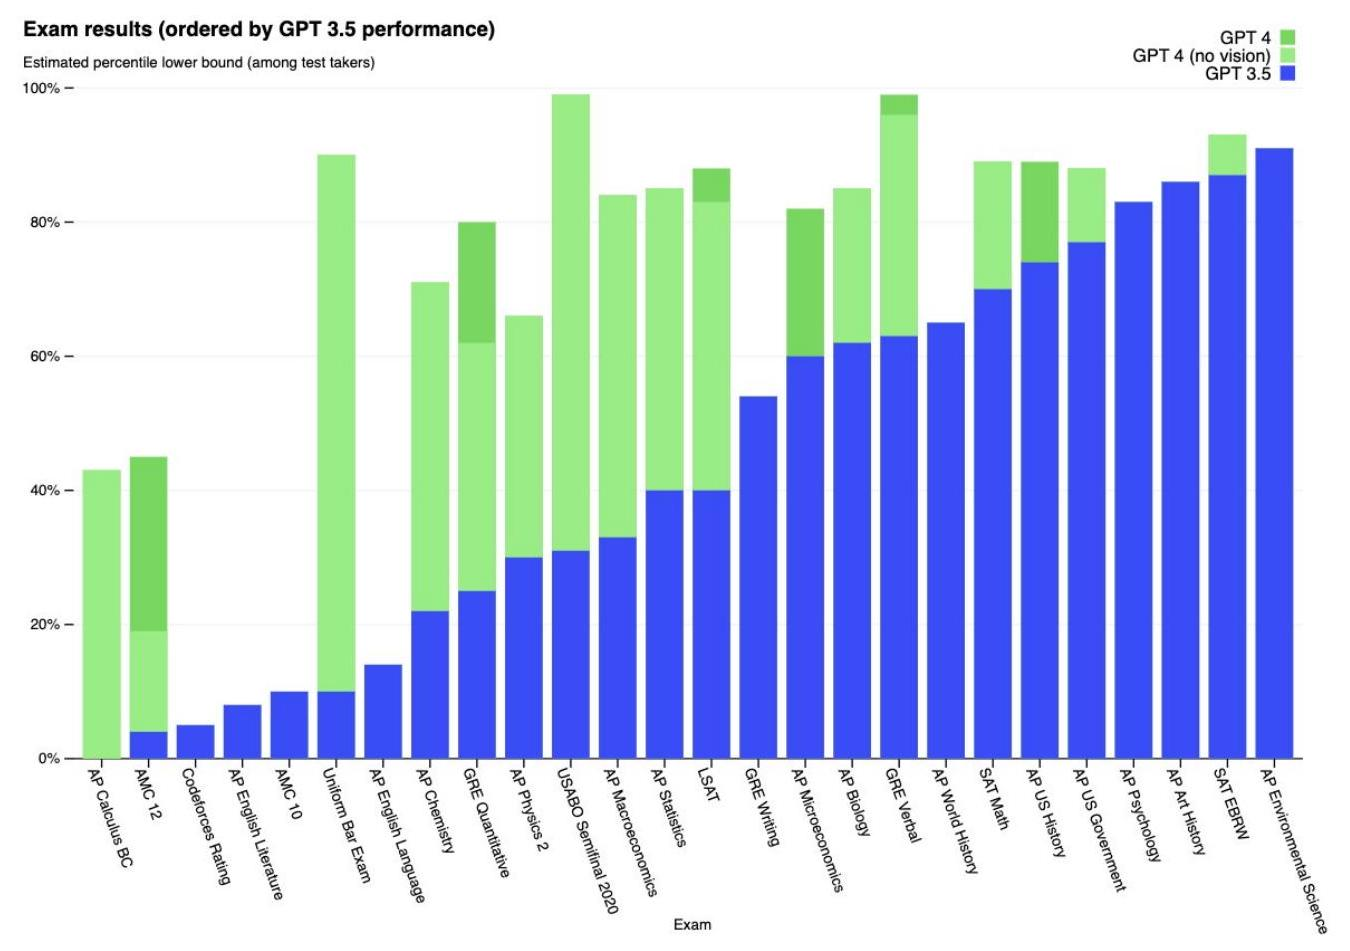
\includegraphics[width=0.90\textwidth]{img/gpt4_technical_report.jpg}
    \caption{Extracted from GPT-4 Technical Report~\cite{openai2023gpt4}. The performance leap between GPT-3.5 and GPT-4 exemplifies the rapid progression in model capabilities~\cite{openai2023gpt4}.}\label{fig:gpt4_technical_report}
\end{figure}

In recent years, generative AI models, particularly large language models (LLMs), have garnered significant attention from both the artificial intelligence (AI) research community and the general public. These models exhibit a remarkable capacity to address a diverse array of intricate language-based tasks. Their advancements are propelled by factors such as increased model parameter count, augmented training data volume, and refined training configurations~\cite{brown2020language, radford2019language, hernandez2021scaling, kaplan2020scaling}. Prominent LLMs like LaMDA~\cite{thoppilan2022lamda} and GPT-4~\cite{openai2023gpt4} demonstrate exceptional proficiency in applications ranging from translation and classification to creative writing and code generation. Such capabilities, previously necessitating task-specific models developed by domain experts using specialized data, are now achieved by these broad, state-of-the-art LLMs.

Concurrently, researchers have enhanced the steerability, reliability, and utility of these models through techniques like fine-tuning and reinforcement learning with human feedback~\cite{ouyang2022training, bai2022training}. These advancements empower models to better understand user intent, thereby enhancing user-friendliness and practicality. Recent studies also showcase LLMs' potential to program and control other digital tools, such as APIs, search engines, and even fellow generative AI systems~\cite{schick2023toolformer, mialon2023augmented}. This integration of individual components facilitates improved utility, performance, and generalization. At the forefront of these trends, there lies a prospect where LLMs can potentially execute any task traditionally performed at a computer.

While generative AI models have primarily been deployed as modular specialists for tasks like image generation from captions or text transcription from speech, the focus is on viewing LLMs as versatile building blocks for creating additional tools. The development and integration of these tools into systems may necessitate time and significant reconfiguration of existing processes across diverse industries. Nevertheless, early adoption trends are already emerging. Despite their limitations, LLMs are increasingly finding integration into specialized applications in areas such as writing assistance, coding, and legal research. These specialized applications enable businesses and individuals to incorporate LLMs into their existing workflows.

The emphasis is on the significance of these complementary technologies, particularly because standalone general-purpose LLMs may still exhibit unreliability for certain tasks, attributable to issues such as factual inaccuracies, inherent biases, privacy concerns, and risks associated with disinformation~\cite{abid2021persistent, schramowski2022large, goldstein2023generative}. However, specialized workflows, encompassing tooling, software, or human-in-the-loop systems, can effectively mitigate these shortcomings by incorporating domain-specific expertise. For instance, Casetext provides LLM-based legal research tools that furnish lawyers with quicker and more accurate legal research results, utilizing embeddings and summarization to counteract the risk of GPT-4 potentially providing inaccurate details about a legal case or set of documents. GitHub Copilot, a coding assistant, leverages LLMs to generate code snippets and auto-complete code, allowing users to accept or reject suggestions based on their expertise. In essence, while GPT-4, on its own, might not inherently `know what time it is,' incorporating a watch can address this limitation.

Moreover, a positive feedback loop may emerge as LLMs surpass specific performance thresholds, enabling them to contribute to the development of tools that enhance their usefulness and usability across diverse contexts. This could potentially reduce the cost and engineering expertise required to create such tools, thereby accelerating LLM adoption and integration~\cite{chen2021evaluating, peng2023impact}. LLMs may also become valuable assets in machine learning model development—serving as coding assistants for researchers.

\subsection{The Impact of Large Language Models on Developer Productivity}
In a recent study~\cite{peng2023impact}, a cumulative total of 166 offers were distributed as part of the experiment, and 95 of these offers were accepted. The 95 developers underwent random assignment into control and treated groups, with 45 individuals in the treated group and 50 in the control group. Thirty-five developers from both the treated and control groups effectively completed the designated task and the subsequent survey.

The majority of the participants fall within the age bracket of $25-34$ and originate from India and Pakistan. This participant cohort is further characterized by a relatively lower income level (median yearly income between $\$10,000-\$19,000$) compared to US standards, yet exhibits a high level of education (with the majority holding a 4-year degree and above). On average, this group possesses six years of coding experience and reports spending approximately 9 hours on coding during a working day.

\begin{figure}[ht]
    \centering
    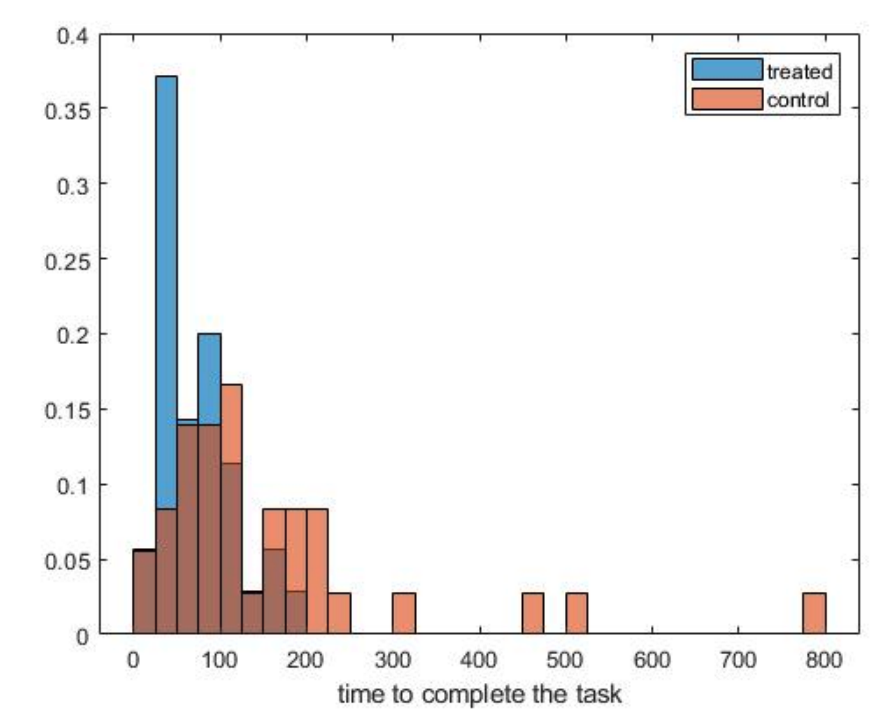
\includegraphics[width=0.8\textwidth]{img/task_completion_time.png}
    \caption{Distribution of time to completion between treated and control groups.}\label{fig:task_completion_time}
\end{figure}

Figure~\ref{fig:task_completion_time} illustrates the distribution of time to completion between the treated and control groups. When conditioned on task completion, the average completion time for the treated group is 71.17 minutes, compared to 160.89 minutes for the control group, resulting in a $55.8\%$ reduction in completion time. The p-value for the t-test is 0.0017, and the $95\%$ confidence interval for the improvement ranges between [21\%, 89\%]. While there are four outliers with completion times exceeding $300 \mathrm{~min}$, all outliers belong to the control group; however, the results remain robust even if these outliers are excluded. This outcome suggests that Copilot significantly enhances average productivity within the experimental population. Additionally, there is a 7 percentage point higher success rate in the treated group compared to the control group, although this estimate lacks statistical significance, with a $95\%$ confidence interval of $[-0.11, 0.25]$.

The exploration then delves into whether this effect varies across different dimensions, including experience, employment status, income, education, and software language preference. The assumption is that the treatment effect is a linear function of the covariates of interest. The results reveal that less experienced developers (in terms of years of professional coding), developers with a heavy coding load (measured in hours of coding per day), and older developers (aged between 25 and 44) derive more significant benefits from Copilot.

To gather insights into the subjects' experiences, an exit survey was conducted with two questions. Initially, participants were asked to estimate the productivity gain or loss (in percentage terms) attributed to Copilot for completing the task. Although the control group was not exposed to Copilot during the task, they were provided with the tutorial video before answering this question to ensure awareness of Copilot features. Figure~\ref{fig:productivity_gain} illustrates the distribution of self-reported productivity gain estimates from both the control and treated groups. On average, participants in both groups estimated a $35 \%$ increase in productivity, which underestimates~\textbf{the actual}~\boldmath{$55.8 \%$}~\textbf{increase in revealed productivity.}

\begin{figure}[ht]
    \centering
    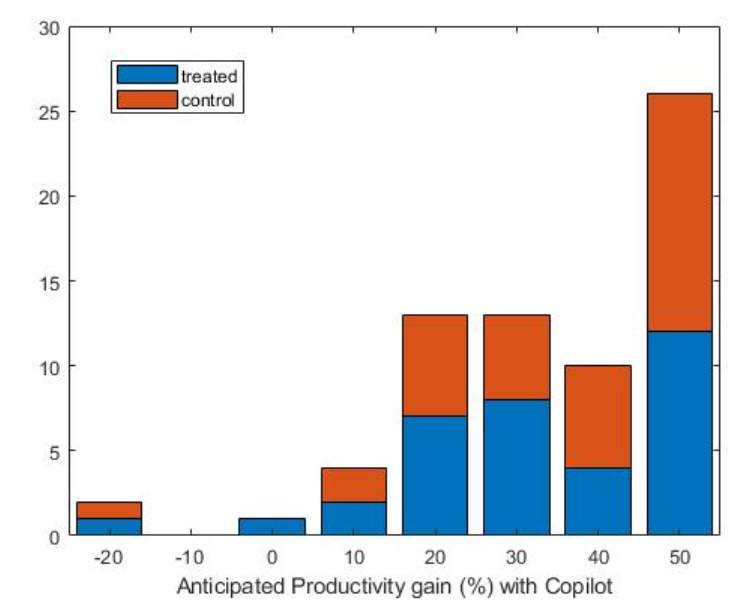
\includegraphics[width=0.8\textwidth]{img/productivity_gain.png}
    \caption{Self-estimated productivity gain.}\label{fig:productivity_gain}
\end{figure}

\section{Theoretical Background}

\subsection{A Taxonomy for Correcting LLMs with Automated Feedback}
For the sake of clean exposition, this survey first presents a conceptual framework outlining the overall process of correcting LLMs with feedback, thereby establishing the scope. It then proceeds to identify five primary dimensions that serve as classification criteria for existing works: 1. What gets corrected, 2. What is the source of the feedback, 3. What is the format of the feedback, 4. When the feedback is used, and 5. How to correct the model with feedback.

\subsubsection{Conceptual Framework}
The general process of correcting LLMs with automated feedback is formulated in Figure~\ref{fig:taxonomy}, using an analogy of medical treatment in daily life. Three parties are involved in this process:

\begin{itemize}
    \item Language Model (Patient). A language model $\mathcal{M}: \mathcal{X} \rightarrow \mathcal{Y}$ performs a specific task by mapping an input $x \in \mathcal{X}$ to an output text $\hat{y} \in \mathcal{Y}$. This formulation encompasses a wide range of NLP tasks. For example, in summarization, $x$ is a passage, $\hat{y}$ is the generated summary; for question-answering, $x$ is a question and $\hat{y}$ is the predicted answer. The initial generation $\hat{y}$ may be imperfect and suffer from various problems such as hallucination and incorrect reasoning.

    \item Critic Model (Doctor \& Diagnosis). A critic model $\mathcal{C}: \mathcal{X} \times \mathcal{Y} \rightarrow \mathcal{F}$ learns to generate feedback $x, \hat{y} \rightarrow c$ where $\hat{y} \sim \mathcal{M}(x)$ is the output or partial output of the language model, and $c$ is the feedback of some format, e.g., scalar value, or natural language. A simple example is binary feedback of whether the output is good or bad given the input $(\mathcal{C}: \mathcal{X} \times \mathcal{Y} \rightarrow\{0,1\})$.

    \item Refine Model (Treatment). A refine model $\mathcal{R}$: $\mathcal{X} \times \mathcal{Y} \times \mathcal{F} \rightarrow \mathcal{Y}$ learns to repair an output $x, \hat{y}, c \rightarrow$ $y_{\text {new }}$ based on the feedback $c$, where $y_{\text {new }}$ is the revised output. Besides repairing output, some refine models directly repair the language model $\mathcal{M}$ through fine-tuning or reinforcement learning.
\end{itemize}

Based on the above formulation, Figure~\ref{fig:taxonomy} illustrates the fundamental interaction among the language model $\mathcal{M}$, the critic model $\mathcal{C}$, and the refine model $\mathcal{R}$. However, the specific model design in existing works varies along five crucial axes, which this survey will elaborate on in the following sections.

\begin{itemize}
    \item Hallucination. An open challenge for LLMs is that they often hallucinate by making up facts or citing sources that do not exist~\cite{li2023halueval, zhang2023language}. These hallucinated contents are often quite plausible-sounding, making it difficult even for humans to detect~\cite{clark2021thats}. To address this, several studies have proposed the collection of automated feedback on potential factual inaccuracies by cross-referencing the output generated by the model with credible knowledge sources. The gathered feedback can then be utilized by a subsequent refinement model to correct hallucinations~\cite{gao2023rarr, zhang2023language}.

    \item Unfaithful Reasoning. LLMs have exhibited a strong ability in solving complex reasoning tasks with improved reasoning strategies, such as Chain-of-Thought prompting~\cite{wei2023chainofthought}. However, recent studies~\cite{golovneva2023roscoe,ribeiro2023street,lyu2023faithful} found that LLMs occasionally make unfaithful reasoning, i.e., the derived conclusion does not follow the previously generated reasoning chain. To address this, existing works have proposed the use of automated feedback from external tools or models for guiding the reasoning process~\cite{xie2023selfevaluation, yao2023tree}, verifying the reasoning process and rectifying errors~\cite{he2022rethinking,pan2023logiclm}, or finetuning LLMs with process-based feedback~\cite{huang2022large, lightman2023lets}.

    \item Toxic, Biased, and Harmful Contents. LLMs have been observed to occasionally generate content that is toxic, biased, or harmful due to biases present in the training data~\cite{shaikh-etal-2023-second}. To rectify this, reinforcement learning from human feedback (RLHF)~\cite{ouyang2022training, bai2022training} has been extensively employed to train LLMs to align more closely with human values, such as being helpful, honest, and harmless. However, RLHF is heavily dependent on highquality human feedback, the collection of which can be resource-intensive. To alleviate this, recent works~\cite{lu2022quark, gou2023critic} have also explored collecting automated feedback to identify and correct potentially harmful outputs.

    \item Flawed Code. Besides generating natural language text, LLMs also show strong abilities to generate computer programs (i.e., code)~\cite{chen2022codet}. However, the generated code can sometimes be flawed or incorrect. To fix this, the approach of learning from automated feedback has been extensively applied in code generation~\cite{chen2023teaching, olausson2023selfrepair}, largely facilitated by the ease of obtaining such feedback through the execution of generated code with the corresponding compilers or interpreters.
\end{itemize}

\begin{figure}[h!]
    \centering
    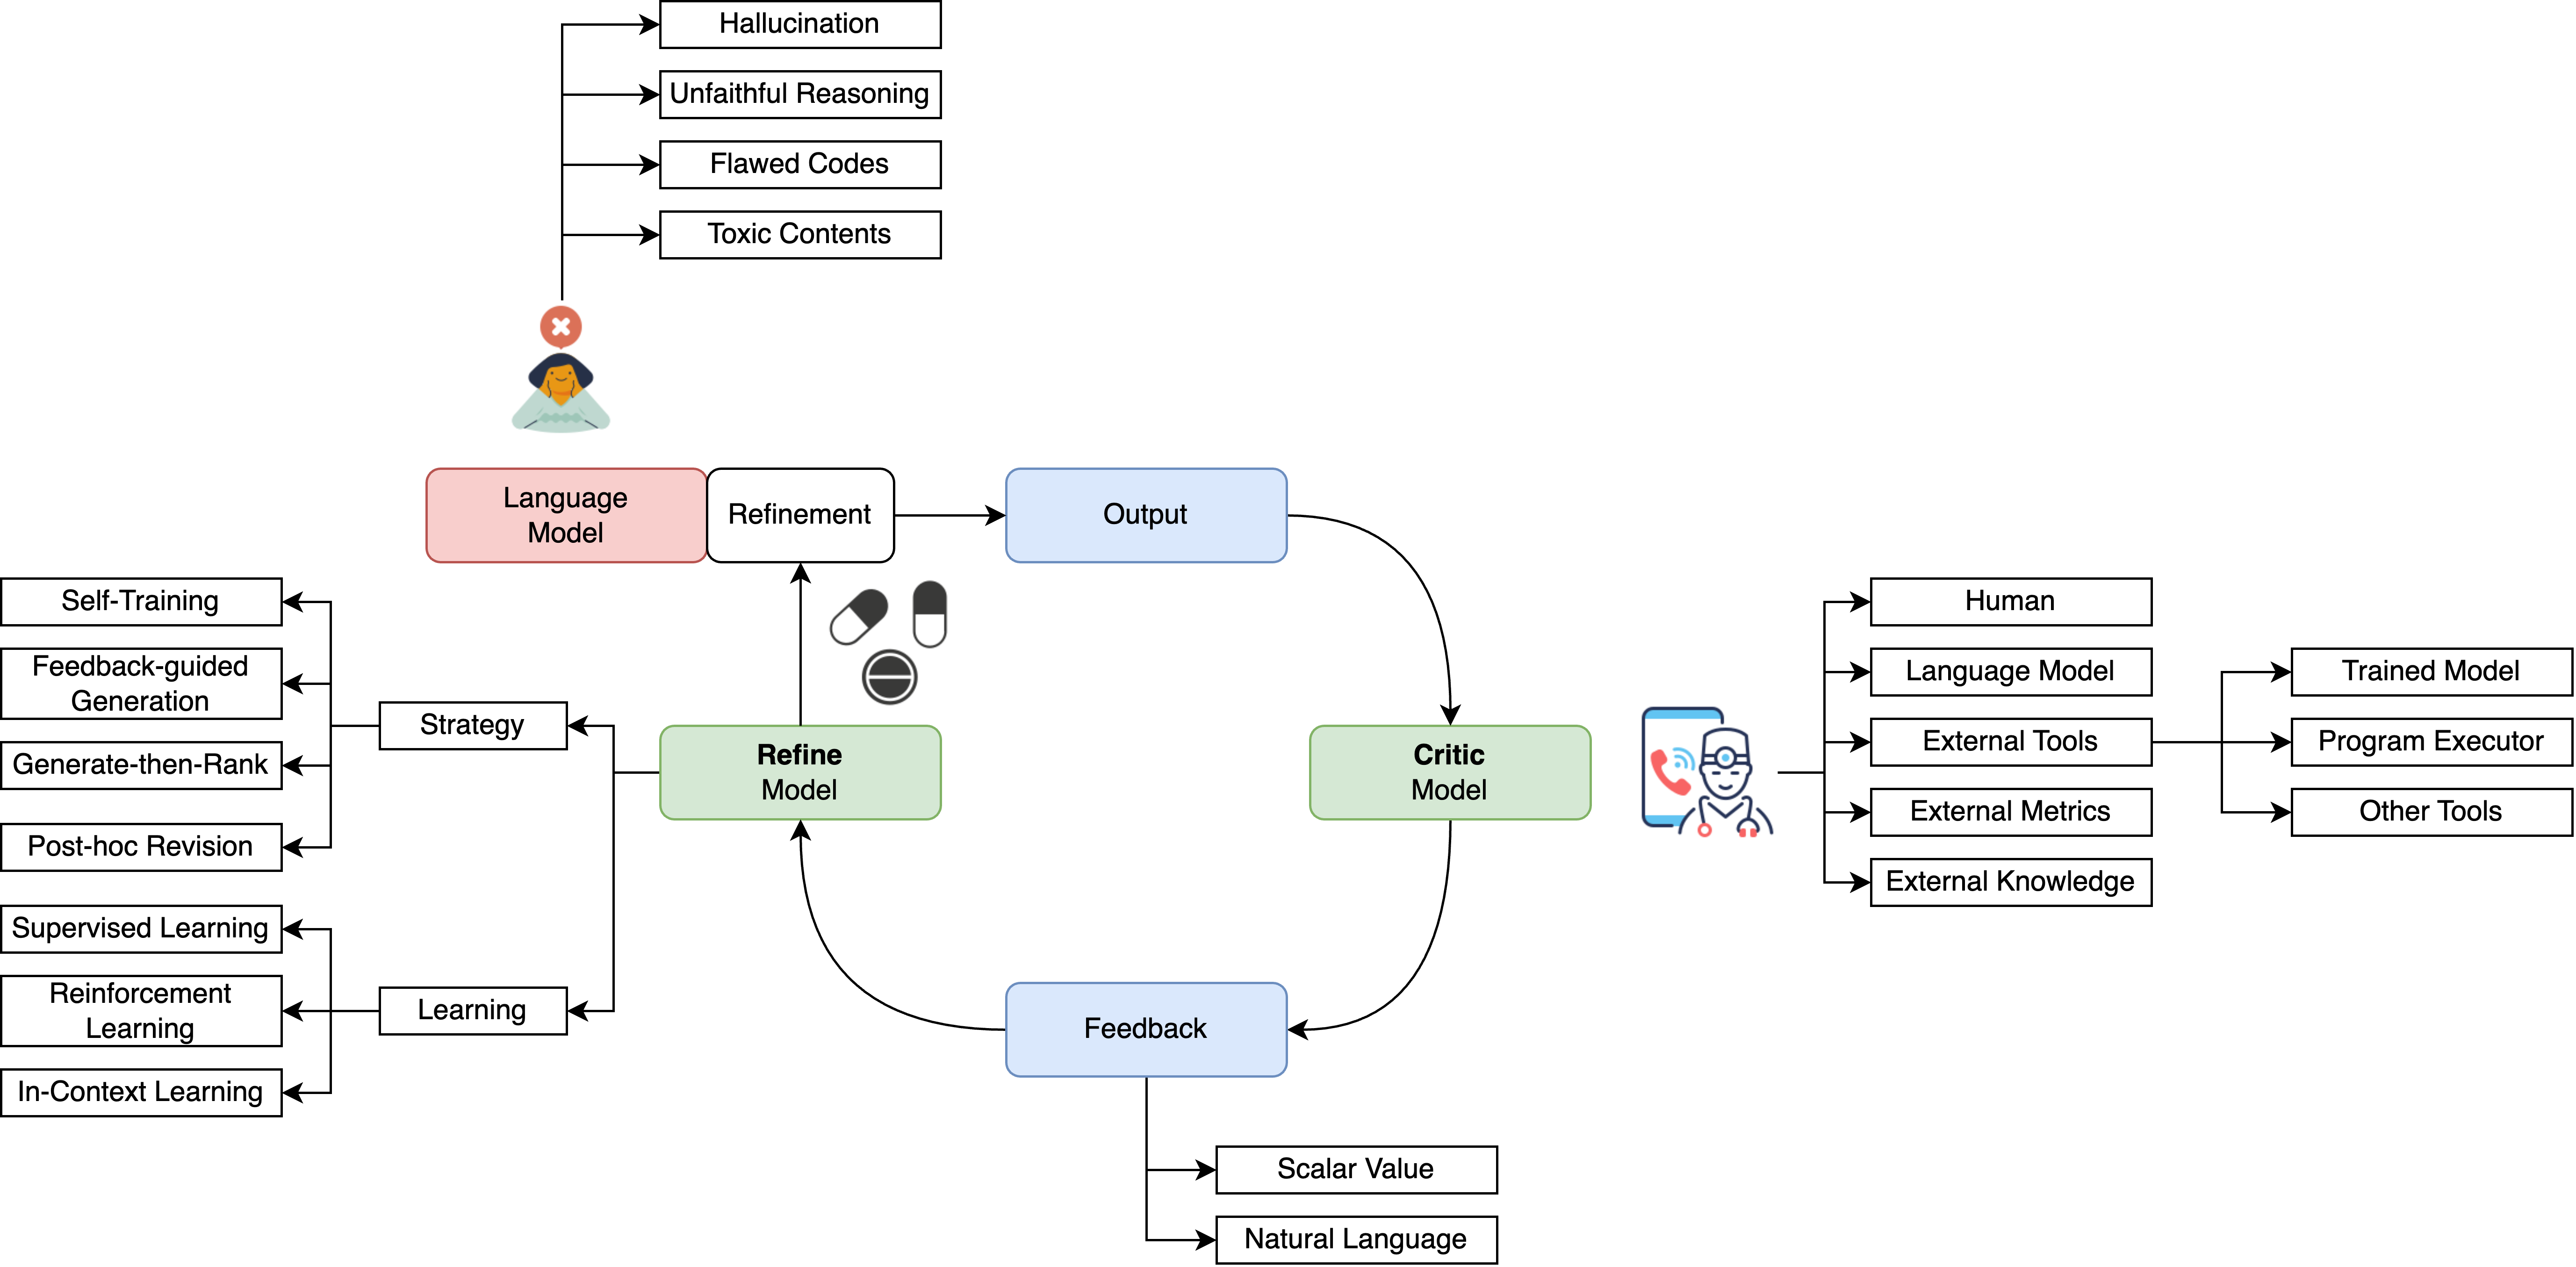
\includegraphics[width=0.90\textwidth]{img/taxonomy.png}
    \caption{A conceptual framework is proposed for self-correcting Language Models (LLMs) with automated feedback. The framework delineates three entities participating in the typical correction pipeline, akin to the roles of a patient, doctor, and treatment in the medical domain. Specifically, a Language Model generates initial output, a Critic Model assesses the output and furnishes feedback, and a Refine Model administers treatment to either the output or the language model. Existing works are categorized using this conceptual framework, addressing five key aspects: the nature of the problem being corrected, the origin and format of the feedback, and the strategy and learning method employed by the refine model.}\label{fig:taxonomy}
\end{figure}

\subsubsection{What is the source of the feedback?}
Feedback can be broadly divided into two categories: human feedback and automated feedback.~\cite{fernandes2023bridging} provided a survey on integrating human feedback for language generation. This survey focuses on the emerging research area of automated feedback, which explores the possibility of LLMs to self-correct without constant human intervention. Automated feedback typically originates from two sources, distinguished by their relationship with the LLM: self-feedback (i.e., the feedback originates from the LLM itself) and external feedback (i.e., the feedback is derived from external models, tools, or knowledge sources).

\begin{itemize}
    \item Self-Feedback. The LLM itself can be utilized as a feedback provider. One straightforward way is to directly evaluate the quality of the generated outputs through prompting and subsequently use this feedback to refine the results~\cite{madaan2023selfrefine, shinn2023reflexion}. This process can be iterative, with the model continually refining its output until it meets a certain standard. This continuous self-improvement strategy has been found particularly useful by numerous studies~\cite{selfee2023, yan-etal-2023-learning}, especially in scenarios where external feedback is unavailable or limited.

    \item External Feedback. Feedback can originate from sources external to the LLM, typically including (1) other trained models~\cite{yan-etal-2023-learning, lightman2023lets}, (2) external tools~\cite{gou2023critic, charalambous2023new}, (3) external knowledge sources~\cite{gao2023rarr, yu2023improving}, and (4) external evaluation metrics~\cite{jung-etal-2022-maieutic, welleck2022generating}. External feedback provides a valuable outside perspective which is particularly useful in identifying errors that the LLM might not recognize on its own. For example, code interpreters are widely used in programming tasks to provide real-time error messages; while external knowledge sources can be utilized to verify the factual accuracy of the LLM's output.
\end{itemize}

\subsubsection{What is the format of the feedback?}
The selection of feedback format requires the consideration of its expressivity, the ease of its collection, and its potential to improve systems~\cite{fernandes2023bridging}. In existing works, automated feedback is typically in the form of a scalar value signal or in natural language.

\begin{itemize}
    \item Scalar Value Feedback. In this scenario, the critic model maps the input and output to a single score $(\mathcal{C}: \mathcal{X} \times \mathcal{Y} \rightarrow \mathcal{N} \subseteq \mathbb{R})$. Scalar value feedback can be easily integrated into the training/decoding process of LLMs. For example, SelfVerification~\cite{weng2023large} ranks candidate outputs to find the optimal one based on the realvalue feedback score assigned by the critic model to each candidate. Similarly,~\cite{xie2023selfevaluation} use real-value feedback for each intermediate reasoning step to guide the model in performing a stochastic beam search for the optimal solution. However, despite its flexibility, scalar value feedback is often less informative to capture detailed information necessary for model correction.

    \item Natural Language Feedback. Natural language feedback offers greater expressivity than scalar value feedback, providing richer information that can highlight the shortcomings of the current output or suggest specific improvements. This form of feedback is particularly crucial for certain applications, such as text editing and code generation. For text editing, PEER~\cite{schick2022peer} trains an LLM to generate detailed suggestions for edits to the initial generated text, such as `remove unsourced claim' or `rewrote the guacamole question for clarity'. For code generation, SelfDebug~\cite{chen2023teaching} uses LLMs to generate explanations for the produced code and utilize both the explanation and the execution results as feedback to enhance coding solutions.
\end{itemize}

\subsubsection{When to correct the model with feedback?}
Depending on the timing of using automated feedback to correct the model, existing works can be divided into three major categories:

\begin{itemize}
    \item Training-time Correction. The ideal scenario is to rectify a flawed model during training, prior to its deployment for use. Once feedback has been collected, it is directly used to optimize the model parameters. Human feedback is typically used for training-time correction, as exemplified by the widely adopted RLHF approach~\cite{ouyang2022training}. For leveraging automated feedback, a common strategy is self-training~\cite{huang2022large}, where the model is trained with its own generated high-quality output filtered by the critic model. While training-time correction is a pre-hoc strategy that addresses problems during training, its practical application may be hindered by: (1) the infeasibility of fine-tuning closed-source LLMs like GPT-4~\cite{openai2023gpt4}, (2) the potential unavailability of feedback during model training, and (3) the requirement for the feedback to be 'optimizable', e.g., a numerical score serving as the basis for model optimization.

    \item Generation-time Correction. This strategy utilizes automated feedback to guide the language model during generation, allowing the model to correct errors in its outputs as it is being generated. For example, for proof generation, several works utilize the automated feedback of the intermediate reasoning steps to guide the model to recover from incorrect generation and search for the optimal solution more efficiently~\cite{yang-etal-2022-generating, lightman2023lets}.

    \item Post-hoc Correction. Finally, post-hoc correction involves refining the model output after it has been generated, without updating the model parameters. This typically involves iteratively generating output, receiving feedback, and refining output. Post-hoc correction provides more flexibility than the previous two strategies as it does not require training the LLM or accessing its parameters. Furthermore, post-hoc correction enhances explainability as it facilitates incorporating more informative natural language feedback. This allows for a more transparent visualization and interpretation of the self-correction process.
\end{itemize}

\subsubsection{How to correct the model with feedback?}
Various concrete strategies have been proposed to correct LLMs with automated feedback, tailored to the different dimensions mentioned in previous sections. For example, self-training is often used for training-time correction. Generate-then-rank often comes with scalar value feedback. Self-refine is the strategy that uses the same LLM as both the critic model and the refine model.

\section{Related Works}
Building upon the taxonomy established in the preceding sections, existing works on correcting LLMs with (automated) feedback are collated in Table 1 and Table 2 based on two major selection criteria:

\begin{enumerate}
    \item Automated Feedback: Explicit feedback is involved to assess the quality of the model output, focusing on automated feedback originating from external models, metrics, knowledge, etc. However, some representative works of human feedback are covered for completeness.

    \item Model Refinement: The feedback acts as a directive to enhance the LLM, either by: (1) updating model parameters, or (2) altering the model's output during or after the generation process.
\end{enumerate}

\subsection{Training-Time Correction}
This section delves into methodologies that rectify model behavior during the training phase. Three typical strategies for training-time correction are identified, each utilizing different forms of feedback to modify the model parameters during training: human feedback, a reward model approximating human feedback, and automated feedback.

\subsubsection{Learning from Human Feedback}
The next-word prediction objective of LLM pretraining is not inherently designed to encapsulate human values or preferences. This misalignment can lead to unintended consequences like generating harmful, misleading, or biased content~\cite{kenton2021alignment}. Many research efforts have explored integrating human feedback to better align LLMs with human values and expectations.~\cite{wang2023aligning} and~\cite{fernandes2023bridging} extensively reviewed this area. However, this survey focuses on automated feedback, so only representative works in this direction are touched upon.

Direct Optimization with Human Feedback. In an ideal scenario, human feedback would directly optimize model parameters. Typically, this approach follows: (1) LLMs generate candidate outputs, (2) Humans provide feedback or refinements on these outputs, and (3) LLMs are optimized on the collected (outputs, feedback) to align with human preferences. One strategy is fine-tuning the model on outputs with positively-labeled feedback. For example, Sparrow~\cite{glaese2022improving} fine-tunes LLMs on dialogues rated as preferred and rule compliant (concerning correctness, harmfulness, and helpfulness) by humans. Similarly,~\cite{scheurer2023training} uses an LLM to generate refinements of the original output based on human feedback, and fine-tunes the original LLM on the best refinement. A similar idea is adopted to fine-tune code generation models~\cite{chen2023improving}. First, human annotators provide feedback for incorrect codes. A refinement model utilizes this to correct the code. Finally, the refined code fine-tunes the code-generating LLM. However, using only positive data (human-refined or positive-rated) may constrain identifying and correcting negative attributes or errors. Chain-of-Hindsight~\cite{liu2023chain} addresses this by fine-tuning the LLM on outputs paired with both positive and negative feedback. Beyond fine-tuning, other optimization methods are explored. For example,~\cite{gao2023continually} uses human feedback as the reward signal and optimizes the model with contextual bandit learning.

Reward Modeling and RLHF. Employing human feedback directly may not always be practical since collecting it can be labor-intensive and time-consuming. An efficient alternative is training a reward model that emulates human feedback. Once trained, this can provide consistent, real-time feedback for every output, circumventing constant human involvement. A prominent example is Reinforcement Learning from Human Feedback (RLHF)~\cite{ouyang2022training}. It first has humans label preference for different LLM outputs and trains the reward model to predict human preference. Then reinforcement learning algorithms (e.g., Proximal Policy Optimization (PPO)~\cite{schulman2017proximal}) optimize the model. RLHF and variants have proven effective in making LLMs more beneficial and less harmful~\cite{bai2022training}, and instilling moral correctness~\cite{ganguli2023capacity}.

\subsubsection{Learning with Automated Feedback}
Since collecting human feedback is resource-intensive, numerous studies have explored using automated feedback to minimize human intervention. Human feedback is defined as a quality assessment by human evaluators on outputs of the base model. This is then used for direct optimization or reward model learning (Section 3.1). Automated feedback is collected offline, without human assessment of model outputs. Two types of automated feedback are discussed: extrinsic from external metrics/models, and intrinsic from the language model itself.

External Metric Guidance. Feedback from external metrics is frequently used for training-time correction. Due to the discrete nature of metric signals, most approaches focus on non-differentiable training techniques. Minimum risk training~\cite{shen-etal-2016-minimum} optimizes parameters with external evaluation metrics~\cite{xu-etal-2022-errors, xu-etal-2023-sescore2}, by incorporating the metric score with

\subsubsection{Feedback-Guided Decoding}
The generate-then-rank method, in which the critic model offers output-level feedback on the entire reasoning path, has certain limitations: (1) The output-level feedback is not fine-grained enough to pinpoint the exact error locations, (2) The extensive length of the output can complicate its quality assessment, and (3) This method does not facilitate fine-grained control over the generation process. For example, the LLM cannot correct its errors during the generation process but must wait until the entire output has been generated.

To address these issues, several works have adopted the feedback-guided decoding strategy, which relies on step-level feedback to offer fine-grained guidance over the generation process. Here, the generation of the output $y$ is broken down into multiple reasoning steps (or thoughts), i.e., $y_{i}=\left[o_{1}, o_{2}, \ldots, o_{n}\right]$. At each individual reasoning step $t$, the critic model provides feedback $\mathcal{C}\left(x, o_{1: t-1}, o_{t}\right)$ that indicates the quality of $o_{t}$ as a candidate step. With the ability to generate and evaluate individual steps, a search algorithm, such as beam search or depth-first search, can be employed for a systematic exploration of the output space, which effectively steers the decoding process toward the generation of an optimal solution. This also allows the LLM to recover from its early mistakes during generation and helps alleviate the reasoning inconsistency problem~\cite{zelikman2022star, creswell2022faithful}, i.e., incorrect reasoning leads to correct final answer.

The feedback-guided decoding strategy has been applied in many recent works, such as Tree-of-Thought~\cite{yao2023tree}, GRACE~\cite{khalifa2023grace}, and RAP~\cite{hao2023reasoning}. These works mostly differ in how to obtain the critic model that provides automated step-level feedback, the most challenging but crucial element of this strategy. The employed methods can be classified into four categories: human feedback, a trained verifier, external metrics, external knowledge, and self-evaluation.

Human feedback can be used to train a step-level reward model, as done by~\cite{uesato2022solving}, who asked annotators to evaluate reasoning steps for problems in GSM8K and trained a binary reward model.~\cite{lightman2023lets} expanded this approach by annotating a larger dataset with 800K human step-level feedback instances. Both studies found step-level feedback assists in training a more reliable reward model, enhancing reasoning faithfulness.

Considering the high cost of human annotations, some works~\cite{yang-etal-2022-generating, tafjord-etal-2022-entailer, li-etal-2023-making, khalifa2023grace} trained a step-wise verifier using synthetic data. Positive examples used groundtruth reasoning paths, while negative examples were created by perturbations.

External metrics have also been used to guide generation, such as minimum Bayes risk decoding to optimize metrics~\cite{freitag-etal-2022-high}, or classifiers to increase likelihood of desired attributes~\cite{dathathri2020plug, yang-klein-2021-fudge, li2022diffusionlm}.

External knowledge can also guide generation, such as using Wikipedia to validate sentences~\cite{varshney2023stitch}, or prior user feedback~\cite{madaan-etal-2022-memory}.

Some works used the LLM itself as the critic via prompting for self-evaluation~\cite{yao2023tree, xie2023selfevaluation}.

Different strategies control decoding given the critic, including search algorithms like beam search~\cite{khalifa2023grace, xie2023selfevaluation}, or Monte Carlo tree search~\cite{zhu-etal-2023-solving, hao2023reasoning}.

\subsection{Generation-Time Correction}
Correcting Language Models (LLMs) during training is often deemed the optimal solution, aligning with the proverbial principle that 'an ounce of prevention is worth a pound of cure.' However, the assurance that all undesired behaviors can be addressed during training is not guaranteed. Furthermore, the correction process during training may be excessively resource-intensive or even impractical for many LLMs, such as closed-source LLMs where weights are inaccessible, and colossal LLMs with billions of parameters. This motivates the exploration of methods seeking to correct LLMs during the generation time or after the output is generated. This section focuses on generation-time correction techniques, where automated feedback serves as a guiding mechanism for LLM generation. Such a strategy allows LLMs to rectify errors during generation without modifying the model parameters. Two primary strategies for generation-time correction are identified: Generate-then-Rank and Feedback-Guided Decoding.

\subsubsection{Generate-then-Rank}
The most immediate strategy involves sampling a large number of candidate generations and subsequently selecting the best generation based on the feedback provided by the critic model. Here, the critic model $\mathcal{C}$ aims to learn the mapping $x, \hat{y}{1}, \ldots, \hat{y}{N} \rightarrow y_{\text {best }}$, where $y_{\text {best }}$ is the best output among the $N$ candidate outputs $\hat{y}{1}, \ldots, \hat{y}{N} \sim \mathcal{M}(x)$.

This approach is often integrated with the Chain-of-Thought (CoT) prompting method~\cite{wei2023chainofthought} to address complex reasoning tasks, such as solving math word problems as demonstrated in GSM8K~\cite{cobbe2021training}. Given an input problem $x$, the LLM initially generates multiple candidate solutions $y_{1}, \ldots, y_{n}$. Each solution $y_{i}=\left[z_{i}, a_{i}\right]$ comprises a reasoning path (explanation) $z_{i}$ leading to the predicted answer $a_{i}$. Subsequently, the critic model $\mathcal{C}$ assigns a plausibility score $s_{i}$ to each candidate reasoning path $z_{i}$. The final selection of the best solution from the scored set $\left(z_{i}, a_{i}, s_{i}\right)_{i=1}^{n}$ is achieved via either ranking or voting.

Various critic models have been proposed in different works. For instance, DIVERSE~\cite{li-etal-2023-making} trains a binary verifier based on DeBERTa~\cite{he2021deberta}, utilizing reasoning paths corresponding to the correct final answer as positive examples and others as negative examples. The best answer is then determined by a majority vote of positively verified candidates.\cite{weng2023large} introduces a training-free critic model based on the idea of self-verification, where the plausibility score is calculated by assessing the consistency between the results of forward reasoning and backward reasoning. In a different vein, RR\cite{he2022rethinking} presents a critic model to assess the faithfulness of each reasoning path by retrieving supporting information from a knowledge base. LEVER~\cite{ni2023lever} applies this strategy in language-to-code generation, with each solution $y_{i}$ serving as a candidate SQL program for the question $x$. A verifier is trained to predict the likelihood of a program's correctness based on the program itself and its execution results. A similar concept is adopted in CodeT~\cite{chen2022codet} where multiple code solutions and test cases are generated by the LLM, and the best code solution is selected through dual execution agreement.

\subsubsection{Feedback-Guided Decoding}
The generate-then-rank method, wherein the critic model offers output-level feedback on the entire reasoning path, encounters certain limitations: 1. The output-level feedback lacks the granularity necessary to pinpoint the exact error locations, 2. The extensive length of the output can complicate its quality assessment, and 3. This method does not facilitate fine-grained control over the generation process. For instance, the Language Model (LM) cannot correct its errors during the generation process but must await the completion of the entire output.

To address these issues, several studies have embraced the feedback-guided decoding strategy, relying on step-level feedback to provide fine-grained guidance over the generation process. Here, the generation of the output $y$ is divided into multiple reasoning steps (or thoughts), i.e., $y_{i}=\left[o_{1}, o_{2}, \ldots, o_{n}\right]$. At each individual reasoning step $t$, the critic model provides feedback $\mathcal{C}\left(x, o_{1: t-1}, o_{t}\right)$ indicating the quality of $o_{t}$ as a candidate step. With the ability to generate and evaluate individual steps, a search algorithm, such as beam search or depth-first search, can be employed for a systematic exploration of the output space, effectively guiding the decoding process toward the generation of an optimal solution. This approach also allows the LM to recover from its early mistakes during generation and helps alleviate the reasoning inconsistency problem~\cite{zelikman2022star, creswell2022faithful}, i.e., incorrect reasoning leading to a correct final answer.

The feedback-guided decoding strategy has found application in recent works, including Tree-of-Thought~\cite{yao2023tree}, GRACE~\cite{khalifa2023grace}, and RAP~\cite{hao2023reasoning}. These works primarily differ in how they obtain the critic model that provides automated step-level feedback, which constitutes the most challenging yet crucial element of this strategy. We classify their employed methods into four categories: human feedback, a trained verifier, external metrics, external knowledge, and self-evaluation.

\begin{itemize}
    \item \textbf{Reward Model from Human Feedback:} One approach involves training a step-level reward model by gathering human feedback.~\cite{uesato2022solving} solicits human annotators to evaluate the correctness of each reasoning step for the problems in GSM8K and subsequently trains a binary reward model.~\cite{lightman2023lets} expands this approach by annotating a larger dataset consisting of 800K instances of human step-level feedback. Both studies discover that step-level feedback assists in training a more reliable reward model, enhancing the faithfulness of reasoning.

    \item \textbf{Training Verifier with Synthetic Data:} Considering the high cost of collecting human annotations and their limited scalability, some works~\cite{yang-etal-2022-generating, tafjord-etal-2022-entailer, li-etal-2023-making, khalifa2023grace} have trained a step-wise verifier using automatically constructed training data. Positive examples are derived from groundtruth reasoning paths, while negative examples are synthesized by proposing an alignment algorithm~\cite{khalifa2023grace} or by making text perturbations on positive samples~\cite{yang-etal-2022-generating}.

    \item \textbf{Feedback from External Metric:} Several works also leverage external metrics to re-rank or guide text generation.~\cite{freitag-etal-2022-high} uses minimum bayes risk decoding on unbiased samples to optimize neural metrics as an alternative to beam search. \textit{Plug and play}~\cite{dathathri2020plug} combines a pretrained model with attribute classifiers that guide text generation without any further training of the model. It leverages the gradient of the classifier to update LM and increase the likelihood of the desirable attribution at the text generation of LM. \textbf{FUDGE}~\cite{yang-klein-2021-fudge} reweights the model predictions at each token and estimates the attribution classification at each partial sequence. Following up on the gradient-based approach, \textbf{DiffusionLM}~\cite{li2022diffusionlm} obtains a sequence of intermediate latent variables by denoising a sequence of Gaussian vectors. It performs iterative gradient updates over latent representations to satisfy controlled requirements from an attribute classifier.

    \item \textbf{Feedback from External Knowledge:} External knowledge sources have also been used to guide the LLM in generation.~\cite{varshney2023stitch} retrieves relevant knowledge from Wikipedia as evidence to validate and correct LLM's generated sentences at each step. Once a non-factual sentence is corrected, the revised sentence is added back to the input along with the prior generations to continue generating the next sentence. In a different approach, \textbf{MemPrompt}~\cite{madaan-etal-2022-memory} leverages prior user feedback as a knowledge source. It maintains an external pool of user feedback and searches it for responses that match the intent of the current query. The retrieved feedback is then concatenated with the input to guide the following generation.

    \item \textbf{Self-Evaluation:} Some studies have utilized a more flexible strategy, employing the LLM itself as the critic model by designing appropriate prompts. For instance, in \textbf{Tree-of-Thought}~\cite{yao2023tree}, the LLM is prompted to assess the value of the current state by producing a scalar value (e.g., $1-10$) or short phrases (e.g., sure/likely/impossible).~\cite{xie2023selfevaluation} employed a similar approach by prompting the LLM with `Is the above step of reasoning: (A) Correct (B) Incorrect'. Self-evaluation provides an efficient evaluation method without requiring task-specific verifier fine-tuning.
\end{itemize}

Existing studies have employed varied strategies to govern the decoding process with the assistance of the step-level critic model. Tree-of-Thought implemented breadth-first search and depth-first search, whereas GRACE~\cite{khalifa2023grace} and~\cite{xie2023selfevaluation} embraced the beam search strategy. In each step, the top-k scoring candidates are chosen for subsequent generations. This iterative process continues until the final answer is generated. Conversely, CoRe~\cite{zhu-etal-2023-solving} and RAP~\cite{hao2023reasoning} opted for the Monte Carlo Tree Search (MCTS) to achieve a suitable equilibrium between exploration and exploitation, enhancing the efficiency of discovering the optimal reasoning path.

\subsection{Post-hoc Correction}
The success of generation-time correction relies on accurate critic feedback for intermediate outputs. However, for holistic tasks like summarization, evaluation requires the full output. Thus, post-hoc correction methods intervene after output generation. Post-hoc correction also allows detailed natural language feedback. Strategies include self-correction, external feedback, and multi-agent debates.


\subsubsection{Self-Correction}
The implementation of post-hoc correction is facilitated through the `Self-Correction' technique, wherein a Language Model (LM) is employed to generate feedback and refine its own output. Initially, an LM is utilized to generate an initial output, and subsequently, the same model serves as a critic to produce feedback and refine this initial output based on the received feedback. This iterative process continues until an output of acceptable quality is achieved or a pre-specified number of iterations are reached.

The Self-Refine framework~\cite{madaan2023selfrefine} proposes a simple yet effective self-correction approach by utilizing a single powerful pre-trained LLM to generate output, provide feedback, and refine the output based on that feedback. All these steps are executed using the same LLM, guided by different prompts. Similarly, in the context of Clinical Self-Verification~\cite{gero2023selfverification}, the self-correction framework is applied to extract patient data from clinical notes. Feedback is generated to identify missing elements in the initially extracted data and to validate the generated data. The output is then refined by eliminating unsupported elements. In contrast, Reflexion~\cite{shinn2023reflexion} emphasizes that prior self-correction research has concentrated on single-turn generation tasks and failed to maintain a record of past errors. To address this, Reflexion proposes the use of the same self-correction framework with the addition of a `long-term memory' capable of storing prior feedback and outputs, thereby preventing the repetition of previous mistakes. Additionally, Reflexion enhances Self-Refine by incorporating scalar-valued feedback and other forms of feedback.

Although self-correction has proven effective for various text-generation tasks, this strategy necessitates the use of powerful, large-scale LLMs capable of refining text based on provided feedback. As noted by~\cite{madaan2023selfrefine}, smaller, open-source models often struggle to refine their output effectively, even when correct feedback is provided. A potential solution involves explicitly training models for this self-correction process. SelFee~\cite{selfee2023} proposes training a model to emulate the self-correction process by generating output, feedback, and a refined solution in an auto-regressive manner. More powerful LLMs are employed to provide feedback and refinement data, with data collection facilitated through ChatGPT.


\subsubsection{Models/Tools as Feedback}
Self-correction relies on language models for feedback, and the quality of this feedback is inherently constrained by the inherent limitations of Language Models (LLMs), such as the inability to access up-to-date information, take actions, or perform precise mathematical reasoning. To overcome these limitations, recent studies have explored the integration of external tools to enhance the feedback provided. Various external tools, including trained models, code interpreters, and search engines, can be incorporated to offer specialized feedback.

Code Interpreter: In code generation, the program executor serves as a feedback source for refining the initial code generated by the model. For instance, Self-Edit~\cite{zhang2023selfedit} and Self-Evolve execute the initial program on example test cases and use the execution results as feedback. Subsequently, an LLM is prompted to refine the initial code based on this feedback. Self-Debug~\cite{chen2023teaching} explores program explanation, unit tests, and program interpreter as feedback types. ALGO~\cite{zhang2023algo} investigates a more fine-grained feedback approach for code generation, generating a reference oracle program for each problem and collecting feedback by comparing outputs from the LLM-generated program with the oracle outputs. The self-correction strategy has also been applied to the formal verification of software, with Bounded Model Checking employed to identify vulnerabilities, followed by LLM-based correction~\cite{charalambous2023new}.

Logic Reasoner: Tool-assisted feedback is utilized to improve the faithfulness of LLMs' reasoning. For example, Logic-LM~\cite{pan2023logiclm} addresses logical reasoning problems by translating them into logical form with LLMs and performing inference with external symbolic solvers. To correct inaccuracies in logical forms, a self-refinement module modifies them using error messages returned by the symbolic reasoner as feedback. Similarly, Baldur~\cite{first2023baldur} utilizes existing search-based proof assistants as a source of feedback to enhance language models' ability to generate theorem proofs.

External Knowledge: External knowledge is frequently integrated as a feedback source to detect and rectify factual errors in LLMs' output and to support LLM-generated facts with evidence or citations. RARR~\cite{gao2023rarr} and REFEED~\cite{yu2023improving} prompt LLMs to raise questions about different aspects of the generated output, and an external retriever searches for evidence to address each query. A refine model then amends the output based on any discrepancies between the output and the retrieved evidence. LLM-Augmenter~\cite{peng2023check} proposes a similar method but differentiates itself by automatically generating natural language feedback based on the retrieved evidence, identifying error locations, and providing revision suggestions. FACTOOL~\cite{chern2023factool} extends knowledge-assisted factual error correction to various tasks, including code generation, mathematical reasoning, and scientific literature review.

Trained Model: Specialized models are fine-tuned for feedback generation, forming a critic that can be paired with similar or more powerful language models in an iterative refinement cycle. CodeRL~\cite{le2022coderl} treats program synthesis as a reinforcement learning task, training a critic model to optimize the main model's output. In contrast, REFINER~\cite{paul2023refiner} trains a task model to produce an intermediate representation, with a critique model providing feedback on each intermediate training step. RLAF~\cite{akyurek-etal-2023-rl4f} employs reinforcement learning to train a critic, keeping the downstream task model fixed, and uses this critic model to produce feedback for the main model. In applications like red-teaming, where vulnerabilities in content filtering systems are targeted, feedback from content filters can guide the generation of better adversarial examples. For instance, Feedback Loop In-context Red Teaming (FLIRT)~\cite{mehrabi2023flirt} uses an explicit image classifier's signal to guide an LLM in producing adversarial input prompts for a text-to-image system, generating more unsafe images for auditing purposes.

Integrating Multiple Tools: Expanding on the concept of tool-assisted feedback, CRITIC~\cite{gou2023critic} integrates various tools in a unified framework, including program interpreters for coding feedback, external knowledge and search engines for factual information, calculators for verifying mathematical equations, and LLM-based natural language feedback. Each tool contributes feedback for different aspects, creating a comprehensive feedback system.

\subsubsection{Multi-Agent Debate}
In addition to the integration of external tools, recent research has investigated the approach of engaging in debates among multiple Language Models (LLMs), inspired by collaborative intelligence, where diverse perspectives often converge toward a more refined solution. This strategy aims to enhance output quality by employing several instances of LLMs. Each instance generates and debates individual responses over multiple rounds to achieve a consensus final answer.

The application and evaluation of this strategy in arithmetic reasoning tasks were first explored by~\cite{du2023improving}. In this context, each agent (a duplicate of an LLM) initially formulates an individual solution along with justifications. The debate phase involves aggregating responses from all agents and presenting this as context to each agent. Based on this context, each agent is then directed to formulate a revised response. The models converge on a shared solution after multiple debate iterations. Experimental results demonstrate that multi-agent debate yields improved performance compared to the self-correction strategy. Expanding on this concept, PRD~\cite{li2023prd} introduced the peer rank algorithm to enhance the consensus-building process after debates. This algorithm considers pairwise preferences between all possible answer pairs from individual LLMs, using these preferences to generate a final ranking of models.

Beyond reasoning tasks, LM vs LM~\cite{cohen2023lm} provided further evidence of the effectiveness of multi-agent debate in detecting factual errors. The approach involves a generator LLM creating a claim, while an examiner LLM probes for factual inaccuracies through a multi-turn interaction. To extend the application of this concept,~\cite{fu2023improving} demonstrated that interactions between different LLMs could simulate human behavior in real-world tasks. The study illustrated this through a bargaining scenario where different LLM agents assumed the roles of buyer and seller. This underscores the versatile applications of multi-agent debates.

\newpage
\bibliography{references}
\bibliographystyle{ieeetr}

\end{document}
